% Options for packages loaded elsewhere
\PassOptionsToPackage{unicode}{hyperref}
\PassOptionsToPackage{hyphens}{url}
%
\documentclass[
  ignorenonframetext,
]{beamer}
\usepackage{pgfpages}
\setbeamertemplate{caption}[numbered]
\setbeamertemplate{caption label separator}{: }
\setbeamercolor{caption name}{fg=normal text.fg}
\beamertemplatenavigationsymbolsempty
% Prevent slide breaks in the middle of a paragraph
\widowpenalties 1 10000
\raggedbottom
\setbeamertemplate{part page}{
  \centering
  \begin{beamercolorbox}[sep=16pt,center]{part title}
    \usebeamerfont{part title}\insertpart\par
  \end{beamercolorbox}
}
\setbeamertemplate{section page}{
  \centering
  \begin{beamercolorbox}[sep=12pt,center]{part title}
    \usebeamerfont{section title}\insertsection\par
  \end{beamercolorbox}
}
\setbeamertemplate{subsection page}{
  \centering
  \begin{beamercolorbox}[sep=8pt,center]{part title}
    \usebeamerfont{subsection title}\insertsubsection\par
  \end{beamercolorbox}
}
\AtBeginPart{
  \frame{\partpage}
}
\AtBeginSection{
  \ifbibliography
  \else
    \frame{\sectionpage}
  \fi
}
\AtBeginSubsection{
  \frame{\subsectionpage}
}
\usepackage{amsmath,amssymb}
\usepackage{lmodern}
\usepackage{iftex}
\ifPDFTeX
  \usepackage[T1]{fontenc}
  \usepackage[utf8]{inputenc}
  \usepackage{textcomp} % provide euro and other symbols
\else % if luatex or xetex
  \usepackage{unicode-math}
  \defaultfontfeatures{Scale=MatchLowercase}
  \defaultfontfeatures[\rmfamily]{Ligatures=TeX,Scale=1}
\fi
% Use upquote if available, for straight quotes in verbatim environments
\IfFileExists{upquote.sty}{\usepackage{upquote}}{}
\IfFileExists{microtype.sty}{% use microtype if available
  \usepackage[]{microtype}
  \UseMicrotypeSet[protrusion]{basicmath} % disable protrusion for tt fonts
}{}
\makeatletter
\@ifundefined{KOMAClassName}{% if non-KOMA class
  \IfFileExists{parskip.sty}{%
    \usepackage{parskip}
  }{% else
    \setlength{\parindent}{0pt}
    \setlength{\parskip}{6pt plus 2pt minus 1pt}}
}{% if KOMA class
  \KOMAoptions{parskip=half}}
\makeatother
\usepackage{xcolor}
\newif\ifbibliography
\usepackage{graphicx}
\makeatletter
\def\maxwidth{\ifdim\Gin@nat@width>\linewidth\linewidth\else\Gin@nat@width\fi}
\def\maxheight{\ifdim\Gin@nat@height>\textheight\textheight\else\Gin@nat@height\fi}
\makeatother
% Scale images if necessary, so that they will not overflow the page
% margins by default, and it is still possible to overwrite the defaults
% using explicit options in \includegraphics[width, height, ...]{}
\setkeys{Gin}{width=\maxwidth,height=\maxheight,keepaspectratio}
% Set default figure placement to htbp
\makeatletter
\def\fps@figure{htbp}
\makeatother
\setlength{\emergencystretch}{3em} % prevent overfull lines
\providecommand{\tightlist}{%
  \setlength{\itemsep}{0pt}\setlength{\parskip}{0pt}}
\setcounter{secnumdepth}{-\maxdimen} % remove section numbering

\usepackage{textpos}
\setbeamertemplate{headline}{
  \begin{textblock*}{5cm}(10.2cm,0.2cm)
  
\includegraphics[width=2.2cm]{UniUrb-logo.png}
  \end{textblock*}}
  
  \definecolor{myblue}{HTML}{005997}
  \setbeamercolor{frametitle}{fg=myblue}
    \setbeamercolor{framesubtitle}{fg=myblue}
    \setbeamercolor{frametitle right}{fg=myblue}
  \setbeamercolor{titlelike}{fg=myblue}
    \setbeamercolor{title}{fg=myblue}
      \setbeamercolor{subtitle}{fg=myblue}
    \setbeamercolor{part title}{fg=myblue}
    \setbeamercolor{section title}{fg=myblue}
    \setbeamercolor{subsection title}{fg=myblue}
  \setbeamercolor{section name}{fg=myblue}
  \setbeamercolor{subsection name}{fg=myblue}
  \setbeamercolor{part name}{fg=myblue}
  \setbeamercolor{title in head/foot}{fg=myblue}
  \setbeamercolor{subtitle in head/foot}{fg=myblue}
  \setbeamercolor{block title}{fg=myblue}
  
  \setbeamercolor{bullet}{fg=myblue}
  \setbeamercolor{section in toc}{fg=myblue}
  \setbeamercolor{subsection in toc}{fg=myblue}
  \setbeamercolor{section in head/foot}{fg=myblue}
  \setbeamercolor{subsection in head/foot}{fg=myblue}
  
  
  \setbeamercolor{itemize item}{fg = myblue}
  \setbeamercolor{itemize subitem}{fg = myblue}
  \setbeamercolor{itemize subsubitem}{fg = myblue}
  \setbeamercolor{enumerate item}{fg = myblue}
  \setbeamercolor{enumerate subitem}{fg = myblue}
  \setbeamercolor{enumerate subsubitem}{fg = myblue}
  
 
  
\usepackage{etoolbox}
\AtBeginEnvironment{thebibliography}{\scriptsize}
\ifLuaTeX
  \usepackage{selnolig}  % disable illegal ligatures
\fi
\usepackage[round]{natbib}
\bibliographystyle{apalike}
\IfFileExists{bookmark.sty}{\usepackage{bookmark}}{\usepackage{hyperref}}
\IfFileExists{xurl.sty}{\usepackage{xurl}}{} % add URL line breaks if available
\urlstyle{same} % disable monospaced font for URLs
\hypersetup{
  pdftitle={Bibliometric Analysis of European Research on Digital Divide: An Exploration of the Corporate Landscape},
  pdfauthor={Luis Carlos Castillo},
  hidelinks,
  pdfcreator={LaTeX via pandoc}}

\title{Bibliometric Analysis of European Research on Digital Divide: An
Exploration of the Corporate Landscape}
\author{Luis Carlos Castillo}
\date{20 March 2023}
\institute{University of Urbino\\
Ph.D.~Program in Global Studies}

\begin{document}
\frame{\titlepage}

\begin{frame}{Content I}
\protect\hypertarget{content-i}{}
\begin{enumerate}
\item
  Motivation
\item
  Objectives
\item
  Digital Divide Overview
\item
  Data
\item
  Bibliometric Analysis
\item
  Performance Analysis

  \begin{enumerate}
  \tightlist
  \item
    Publications Vs Citations
  \item
    Authors
  \item
    Articles
  \item
    Journals
  \item
    Affiliations/ Universities
  \item
    Countries
  \end{enumerate}
\end{enumerate}
\end{frame}

\begin{frame}{Content II}
\protect\hypertarget{content-ii}{}
\begin{enumerate}
\setcounter{enumi}{6}
\item
  Science Mapping

  \begin{enumerate}
  \tightlist
  \item
    Citations Analysis
  \item
    Similarity Measures

    \begin{enumerate}
    \tightlist
    \item
      Co-citations Analysis
    \item
      Bibliographic Coupling
    \item
      Co-word Analysis
    \end{enumerate}
  \end{enumerate}
\end{enumerate}
\end{frame}

\begin{frame}{1. Motivation}
\protect\hypertarget{motivation}{}
\begin{itemize}
\item
  The ubiquitous use of digital technologies has transformed many
  aspects of society and the economy, bringing potential benefits and
  drawbacks.
\item
  The Digital Europe program and the agenda to bridge the digital
  divide.
\item
  The few studies using the bibliometric method focus mainly on health
  sciences, computer science, and technology.
\item
  Data availability from three platforms containing references and
  citations from academic journals has stimulated this research
  initiative.
\end{itemize}
\end{frame}

\begin{frame}{2. Objectives and Research Questions I}
\protect\hypertarget{objectives-and-research-questions-i}{}
\begin{block}{Objectives}
\protect\hypertarget{objectives}{}
\begin{itemize}
\item
  Understand the intellectual structure within the domain of the digital
  divide.
\item
  Examine European research components' intellectual interactions,
  structural connections, and thematic relationships.
\item
  Explore the corporate digital divide among the collected corpus and
  identify trends and patterns within the literature.
\end{itemize}
\end{block}
\end{frame}

\begin{frame}{2. Objectives and Research Questions II}
\protect\hypertarget{objectives-and-research-questions-ii}{}
\begin{block}{Research Questions}
\protect\hypertarget{research-questions}{}
\begin{itemize}
\item
  What have been the main trends and shifts in the focus of European
  research on the digital divide over time?
\item
  Which are the most prominent authors and publications in the field?
\item
  How do the intellectual interactions, structural connections, and
  thematic relationships among European research components on the
  digital divide shape the current state of knowledge in this field?
\item
  What are the key themes and subtopics related to the digital divide in
  European research, and how are they grouped or clustered in the
  literature?
\item
  How is the corporate digital divide addressed in European research on
  the digital divide, and what areas have been largely unexplored in
  this field?
\end{itemize}
\end{block}
\end{frame}

\begin{frame}{3. The Digital Divide Overview I}
\protect\hypertarget{the-digital-divide-overview-i}{}
\begin{itemize}
\tightlist
\item
  The digital divide is also known as the digital gap, inequalities, or
  disparities.
\item
  The interaction with other existing gaps such as income, education,
  gender, generational, and regional, among others \citep{ragnedda2017}.
\item
  The evolution of the concept has pointed out the phenomenon's
  complexity and the effects on the different layers of society and the
  economy \citep{vandijk2003, ragnedda2017, shakina2021}.
\end{itemize}
\end{frame}

\begin{frame}{3. The Digital Divide Overview II}
\protect\hypertarget{the-digital-divide-overview-ii}{}
\begin{itemize}
\tightlist
\item
  Waves of Research

  \begin{itemize}
  \item
    \textbf{The first wave:} Physical access to technology
    -\textgreater{} possession of computers and access to the internet
    \citep{vandijk2003}.
  \item
    \textbf{The second wave:} Usage of digital technologies and skills
    \citep{vandijk2006}.
  \item
    The divide is not exclusively a matter of access or possession of
    technology. It encloses the ability to effectively search, access,
    and evaluate information using digital technologies.
  \end{itemize}
\end{itemize}
\end{frame}

\begin{frame}{3. The Digital Divide Overview III}
\protect\hypertarget{the-digital-divide-overview-iii}{}
\begin{itemize}
\tightlist
\item
  Waves of Research

  \begin{itemize}
  \item
    \textbf{The third wave:} expands upon the inequalities previously
    identified in the 1st and 2nd wave.
  \item
    Focuses on the benefits previously gained from access, skills, and
    usage of digital technologies.
  \item
    Emphasize on the ability to benefit from digital technologies in a
    data-driven market to improve personal and professional aspects
    \citep{ragnedda2017}.
  \item
    van Deursen et al.~(2015) highlight the disparities from the
    tangible outcomes gained from different forms of access and usage of
    digital technologies.
  \end{itemize}
\end{itemize}
\end{frame}

\begin{frame}{3. The digital divide overview VI}
\protect\hypertarget{the-digital-divide-overview-vi}{}
\begin{block}{The corporate landscape}
\protect\hypertarget{the-corporate-landscape}{}
\begin{itemize}
\tightlist
\item
  Digital revolution -\textgreater{} different aspects of daily
  activities -\textgreater{} how we conduct business.
\item
  The corporate digital divide is the disparity in digital capabilities
  and resources between businesses that can effectively use DT and those
  that struggle to access and use it \citep{shakina2021}.
\item
  The corporate digital divide occurs at the regional, industry-type,
  and business-size levels \citep{pejicbach2013}. Usage gap
  \citep{pliskin2006}.
\end{itemize}
\end{block}
\end{frame}

\begin{frame}{3. The digital divide overview VI}
\protect\hypertarget{the-digital-divide-overview-vi-1}{}
\begin{block}{The corporate landscape: research in Europe}
\protect\hypertarget{the-corporate-landscape-research-in-europe}{}
\begin{itemize}
\tightlist
\item
  Out of 1641 articles retrieved, a second search within this sample
  found 32 articles addressing the corporate digital divide.
\item
  Period 2000-2007: refers to the digital gap among firms sizes,
  especially in the access to - ICT and the implementation of
  e-business.
\end{itemize}
\end{block}
\end{frame}

\begin{frame}{3. The digital divide overview VII}
\protect\hypertarget{the-digital-divide-overview-vii}{}
\begin{block}{The corporate landscape: research in Europe}
\protect\hypertarget{the-corporate-landscape-research-in-europe-1}{}
\begin{itemize}
\tightlist
\item
  Period 2008-2015: the focus shifted to analyzing firm readiness for
  digital technologies and skills. It also identified the factors that
  contribute to the digital divide among businesses.
\item
  Period 2000-2022: emphasize digital skills and the advantages of DT.
  It also shows evidence from different countries.
\end{itemize}
\end{block}
\end{frame}

\begin{frame}{4. Data I}
\protect\hypertarget{data-i}{}
\begin{itemize}
\tightlist
\item
  Specific search within titles and author keywords on the
  ``\emph{digital divide}'' merging data from the Web of Science,
  Scopus, and Dimensions platforms.
\item
  Search criteria: ``digital divide*'' OR ``digital inequalit*'' OR
  ``digital gap*''
\item
  The sample includes articles, book chapters, conferences, and
  proceedings.
\item
  Authors with European affiliations within the business, management,
  economics, technology, and computer science disciplines were included
\end{itemize}
\end{frame}

\begin{frame}{4. Data II}
\protect\hypertarget{data-ii}{}
\begin{itemize}
\item
  After conducting a thorough data cleaning, a total of 1641 unique
  documents from 2000 to 2022 were incorporated.
\item
  To track the evolution of the digital divide literature, the data was
  divided into three periods: 2000-2007, 2008-2015, and 2016-2022.
\item
  Document distribution

  \begin{itemize}
  \tightlist
  \item
    WoS:946
  \item
    Scopus: 286
  \item
    Dimensions: 409
  \end{itemize}
\item
  The R programming language environment was used to carry out the
  analysis.
\end{itemize}
\end{frame}

\begin{frame}{5. Bibliometric Analysis I}
\protect\hypertarget{bibliometric-analysis-i}{}
Following \citet{donthu2021}, \citet{Aria2017}, \citet{ellegaard2015}
and \citet{Bornmann2015} bibliometric analysis:

\begin{itemize}
\tightlist
\item
  Is a methodology that applies quantitative techniques to bibliographic
  data and plays a vital role in evaluating research output.
\item
  This technique allows researchers to uncover emerging trends
  identifying knowledge gaps in specific domains.
\item
  Is useful when analyzing a significant quantity of documents.
\item
  It offers three types of analysis: performance analysis, science
  mapping, and network analysis.
\end{itemize}
\end{frame}

\begin{frame}{5. Bibliometric Analysis II}
\protect\hypertarget{bibliometric-analysis-ii}{}
\begin{block}{Descriptive Analysis}
\protect\hypertarget{descriptive-analysis}{}
\begin{table}
\centering
\resizebox{\linewidth}{!}{
\begin{tabular}{l|l|l|l|l}
\hline
\textbf{Details} & \textbf{Period.1} & \textbf{Period.2} & \textbf{Period.3} & \textbf{Total}\\
\hline
Timespan & 2000 - 2007 & 2008 - 2015 & 2016 - 2022 & 2000 - 2022\\
\hline
Journals & 123 & 301 & 533 & 848\\
\hline
Annual growth rate & 71.14 & 3.94 & 15.77 & 26.72\\
\hline
Average citations per doc & 42.87 & 23.29 & 10.37 & 18.49\\
\hline
Total published documents & 202 & 523 & 916 & 1641\\
\hline
Articles & 159 & 354 & 748 & 1261\\
\hline
Book chapters & 4 & 34 & 17 & 55\\
\hline
Porceeding papers & 35 & 93 & 107 & 235\\
\hline
Conference papers & 4 & 42 & 44 & 90\\
\hline
\end{tabular}}
\end{table}
\end{block}
\end{frame}

\begin{frame}{6. Performance Analysis I}
\protect\hypertarget{performance-analysis-i}{}
\begin{block}{6.1. Publications vs Citations}
\protect\hypertarget{publications-vs-citations}{}
\vspace{0.5cm}

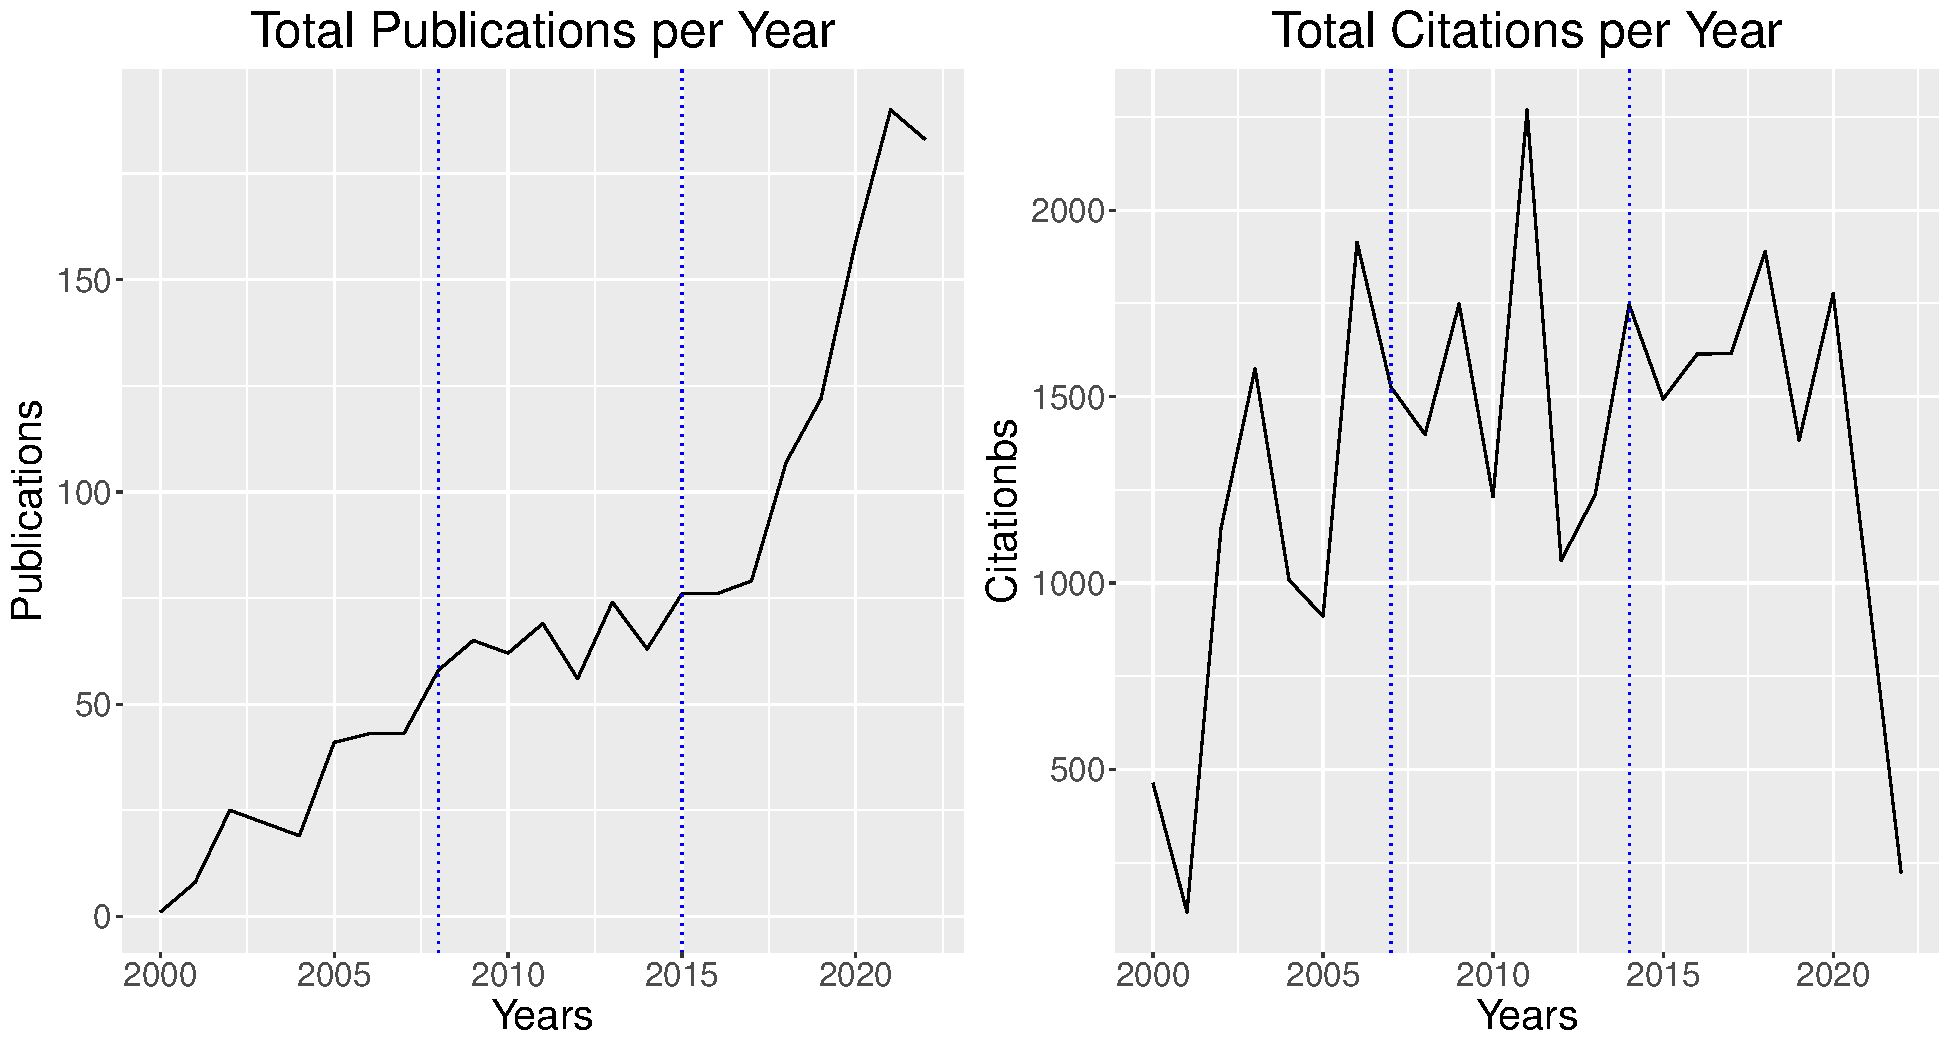
\includegraphics{Presentation_bibliometric_files/figure-beamer/Panel cite vs prod-1.pdf}
\end{block}
\end{frame}

\begin{frame}{6. Performance Analysis I}
\protect\hypertarget{performance-analysis-i-1}{}
\vspace{0.5cm}

\begin{block}{6.2. Evolving patterns in authors' scientific production
over time.}
\protect\hypertarget{evolving-patterns-in-authors-scientific-production-over-time.}{}
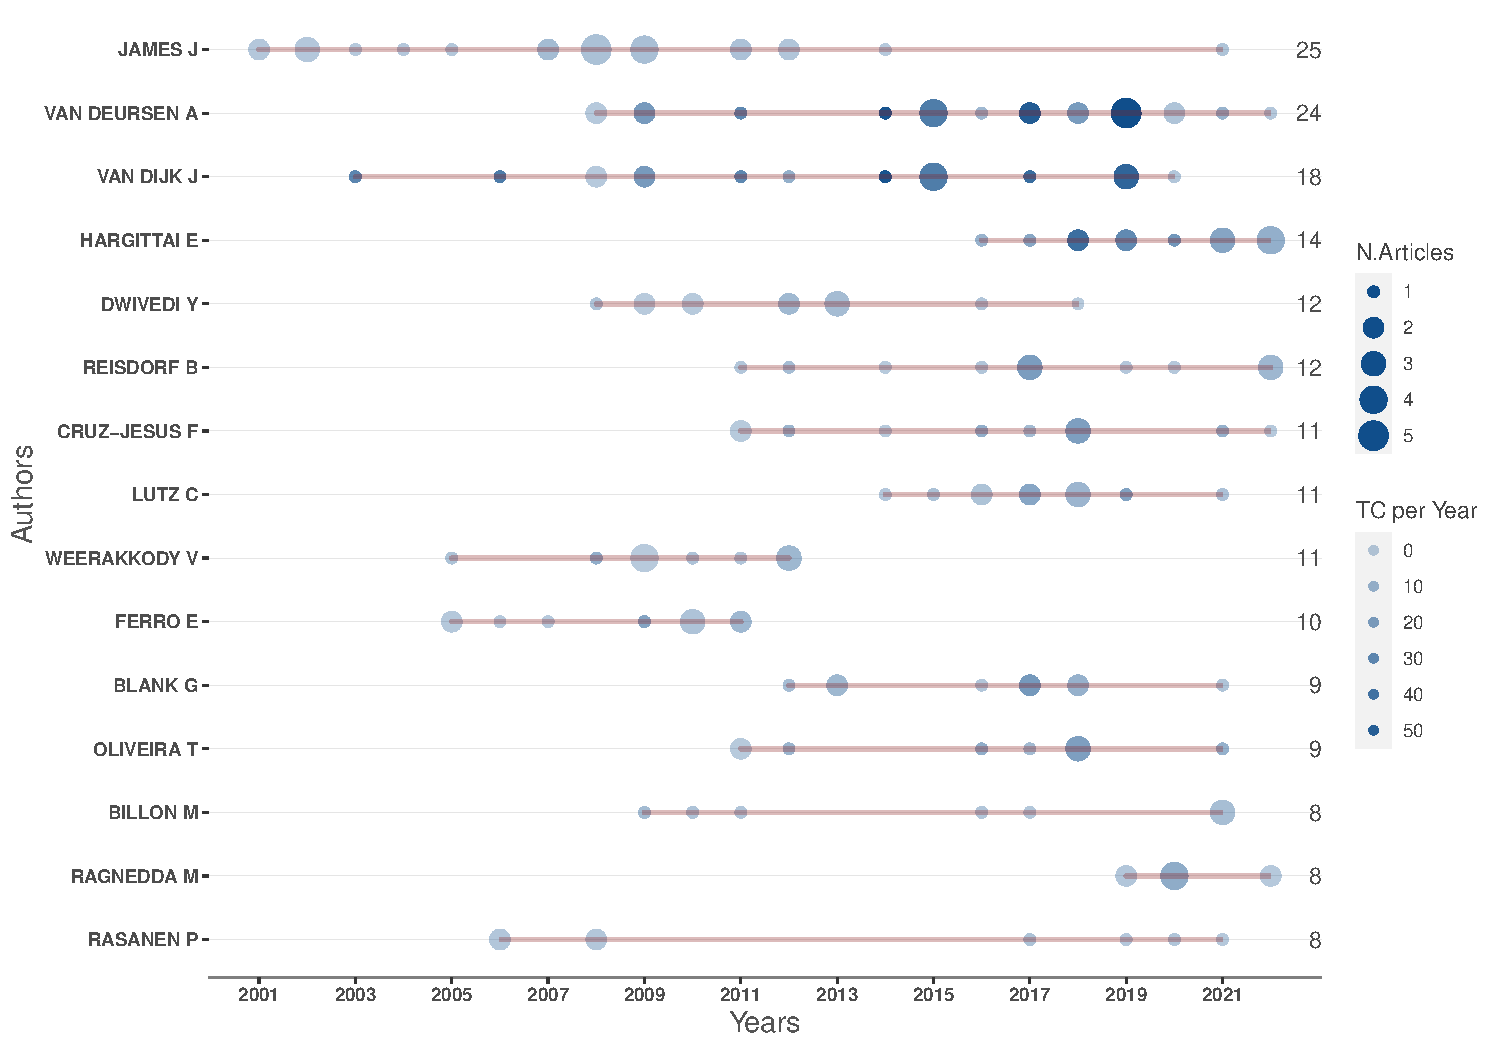
\includegraphics{Presentation_bibliometric_files/figure-beamer/Prod of AU-1.pdf}
\end{block}
\end{frame}

\begin{frame}{6. Performance Analysis}
\protect\hypertarget{performance-analysis}{}
\begin{block}{6.2. Trends in authors' citations over time}
\protect\hypertarget{trends-in-authors-citations-over-time}{}
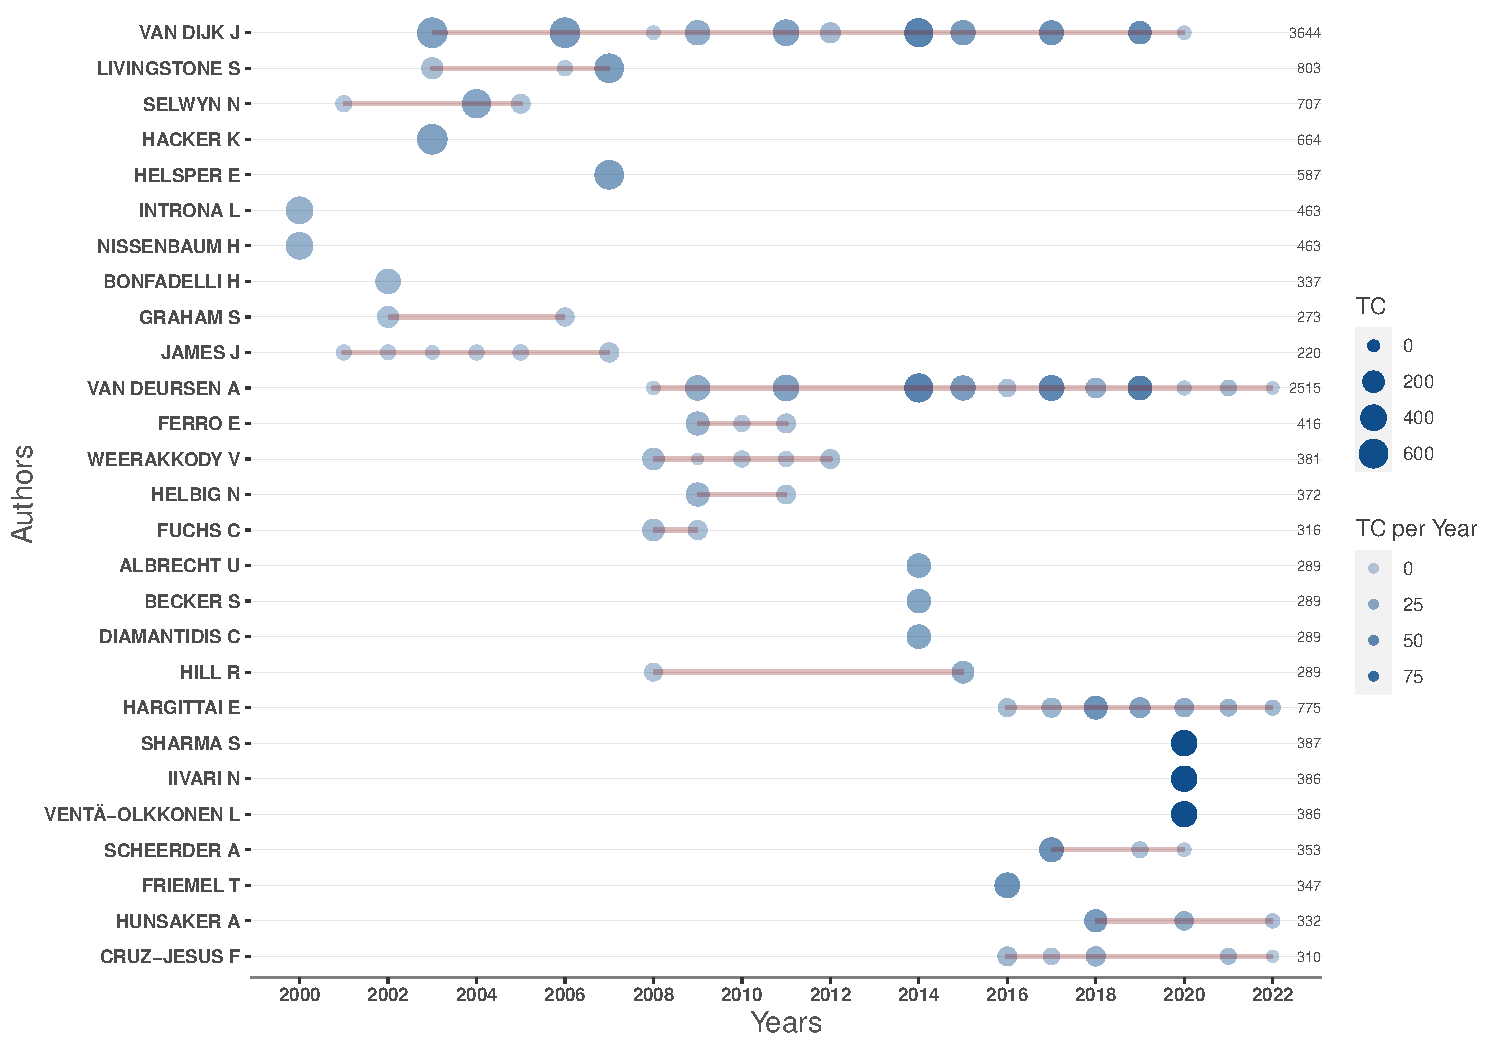
\includegraphics{Presentation_bibliometric_files/figure-beamer/Influence of AU chart-1.pdf}
\end{block}
\end{frame}

\begin{frame}{6. Performance Analysis}
\protect\hypertarget{performance-analysis-1}{}
\begin{block}{6.2. Authors II}
\protect\hypertarget{authors-ii}{}
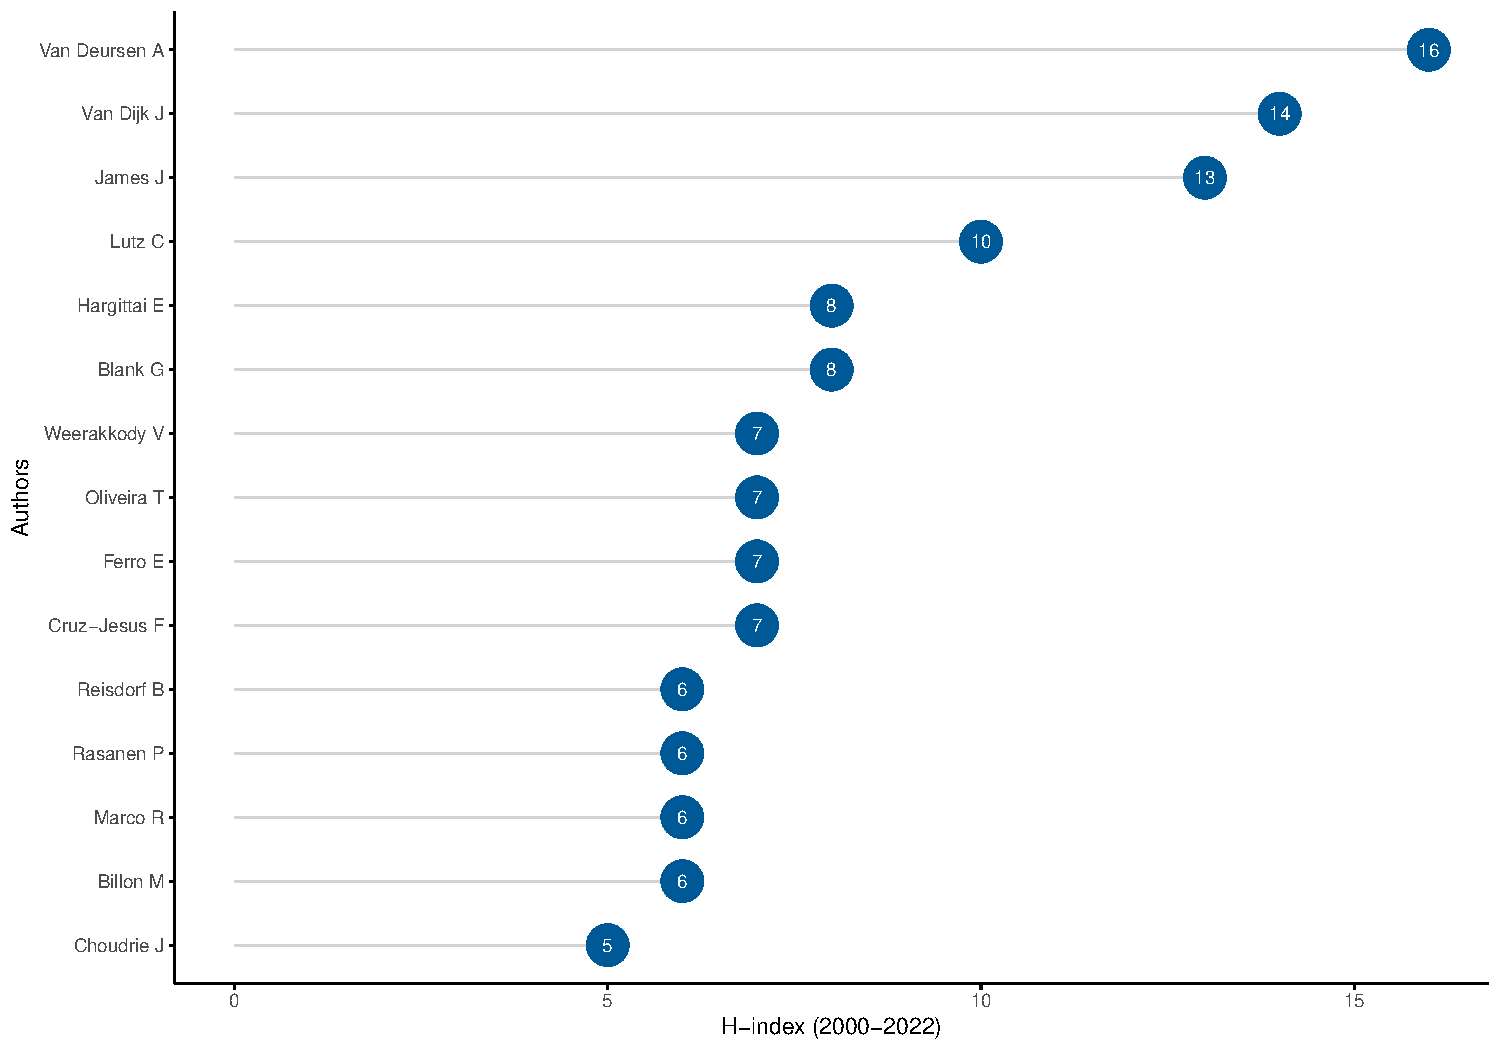
\includegraphics{Presentation_bibliometric_files/figure-beamer/H-index AU chart-1.pdf}
\end{block}
\end{frame}

\begin{frame}{6. Performance Analysis}
\protect\hypertarget{performance-analysis-2}{}
\begin{block}{6.3. Articles I}
\protect\hypertarget{articles-i}{}
\begin{table}

\caption{\label{tab:Influence of AU table }Most Cited Articles}
\centering
\fontsize{5}{7}\selectfont
\begin{tabular}[t]{r|p{9cm}|r}
\hline
\textbf{Rank} & \textbf{Article} & \textbf{TC}\\
\hline
\multicolumn{3}{c}{\textbf{Period 1: 2000- 2007}}\\
\hline
\hspace{1em}1 & Van Dijk J; Hacker K (2003) -The Digital Divide As A Complex And Dynamic Phenomenon & 664\\
\hline
\hspace{1em}2 & Van Dijk J (2006) -Digital Divide Research, Achievements And Shortcomings & 660\\
\hline
\hspace{1em}3 & Livingstone S; Helsper E (2007) -Gradations In Digital Inclusion: Children, Young People And The Digital Divide & 587\\
\hline
\hspace{1em}4 & Selwyn N (2004) -Reconsidering Political And Popular Understandings Of The Digital Divide & 560\\
\hline
\hspace{1em}5 & Introna L; Nissenbaum H (2000) -Shaping The Web: Why The Politics Of Search Engines Matters & 463\\
\hline
\multicolumn{3}{c}{\textbf{Period 2: 2008- 2015}}\\
\hline
\hspace{1em}1 & Van Deursen A; Van Dijk J (2014) -The Digital Divide Shifts To Differences In Usage & 555\\
\hline
\hspace{1em}2 & Van Deursen A; Van Dijk J (2011) -Internet Skills And The Digital Divide & 402\\
\hline
\hspace{1em}3 & Becker S; Miron-Shatz T; Schumacher N; Krocza J; Diamantidis C; Albrecht U (2014) -Mhealth 2.0: Experiences, Possibilities, And Perspectives & 289\\
\hline
\hspace{1em}4 & Helbig N; Gil-García J; Ferro E (2009) -Understanding The Complexity Of Electronic Government: Implications From The Digital Divide Literature & 268\\
\hline
\hspace{1em}5 & Carter L; Weerakkody V (2008) -E-Government Adoption: A Cultural Comparison & 208\\
\hline
\multicolumn{3}{c}{\textbf{Period 3: 2016- 2022}}\\
\hline
\hspace{1em}1 & Iivari N; Sharma S; Ventä-Olkkonen L (2020) -Digital Transformation Of Everyday Life – How Covid-19 Pandemic Transformed The Basic Education Of The Young Generation And Why Information Management Research Should Care? & 386\\
\hline
\hspace{1em}2 & Friemel T (2016) -The Digital Divide Has Grown Old: Determinants Of A Digital Divide Among Seniors & 347\\
\hline
\hspace{1em}3 & Scheerder A; Van Deursen A; Van Dijk J (2017) -Determinants Of Internet Skills, Uses And Outcomes. A Systematic Review Of The Second- And Third-Level Digital Divide & 307\\
\hline
\hspace{1em}4 & Hunsaker A; Hargittai E (2018) -A Review Of Internet Use Among Older Adults & 223\\
\hline
\hspace{1em}5 & Van Deursen A; Van Dijk J (2019) -The First-Level Digital Divide Shifts From Inequalities In Physical Access To Inequalities In Material Access & 198\\
\hline
\multicolumn{3}{l}{\textsuperscript{1} Source: Author's elaboration}\\
\multicolumn{3}{l}{\textsuperscript{2} TC: Times Cited}\\
\end{tabular}
\end{table}
\end{block}
\end{frame}

\begin{frame}{6. Performance Analysis}
\protect\hypertarget{performance-analysis-3}{}
\begin{block}{6.3. Articles II}
\protect\hypertarget{articles-ii}{}
\end{block}
\end{frame}

\begin{frame}{6. Performance Analysis}
\protect\hypertarget{performance-analysis-4}{}
\begin{block}{6.4. Journals}
\protect\hypertarget{journals}{}
\begin{table}

\caption{\label{tab:Influencial SO}Journals' Performance}
\centering
\fontsize{8}{10}\selectfont
\begin{tabular}[t]{r|l|r|r}
\hline
\textbf{Rank} & \textbf{Journals} & \textbf{TC} & \textbf{PD}\\
\hline
1 & New Media \& Society & 4427 & 42\\
\hline
2 & Information Society & 2066 & 26\\
\hline
3 & Information Communication \& Society & 1165 & 43\\
\hline
4 & Government Information Quarterly & 965 & 15\\
\hline
5 & Telecommunications Policy & 961 & 34\\
\hline
6 & Poetics & 945 & 6\\
\hline
7 & Telematics And Informatics & 921 & 21\\
\hline
8 & Computers In Human Behavior & 837 & 15\\
\hline
9 & Universal Access In The Information Society & 590 & 15\\
\hline
10 & European Journal Of Communication & 447 & 6\\
\hline
\multicolumn{4}{l}{\textsuperscript{1} Source: Author's elaboration}\\
\multicolumn{4}{l}{\textsuperscript{2} TC: Times Cited}\\
\multicolumn{4}{l}{\textsuperscript{3} PD: Published Documents}\\
\end{tabular}
\end{table}
\end{block}
\end{frame}

\begin{frame}{6. Performance Analysis}
\protect\hypertarget{performance-analysis-5}{}
\begin{block}{6.5. Affiliations/ Universities}
\protect\hypertarget{affiliations-universities}{}
\begin{table}

\caption{\label{tab:Influencial UN}Top 10 University's Performance}
\centering
\fontsize{8}{10}\selectfont
\begin{tabular}[t]{r|l|r|r}
\hline
\textbf{Rank} & \textbf{University} & \textbf{TC} & \textbf{PD}\\
\hline
1 & Univ Twente & 4085 & 31\\
\hline
2 & London Sch Econ And Polit Sci & 2195 & 24\\
\hline
3 & Univ Zurich & 1581 & 26\\
\hline
4 & Univ Oxford & 1037 & 38\\
\hline
5 & Cardiff Univ & 793 & 10\\
\hline
6 & New Mexico State Univ & 664 & 1\\
\hline
7 & Brunel Univ London London & 660 & 15\\
\hline
8 & Univ Oviedo & 526 & 10\\
\hline
9 & Univ Loughborough & 501 & 16\\
\hline
10 & Tilburg Univ & 464 & 29\\
\hline
\multicolumn{4}{l}{\textsuperscript{1} Source: Author's elaboration}\\
\multicolumn{4}{l}{\textsuperscript{2} TC: Times Cited}\\
\multicolumn{4}{l}{\textsuperscript{3} PD: Published Documents}\\
\end{tabular}
\end{table}
\end{block}
\end{frame}

\begin{frame}{6. Performance Analysis}
\protect\hypertarget{performance-analysis-6}{}
\begin{block}{6.5. Countrys' Performance}
\protect\hypertarget{countrys-performance}{}
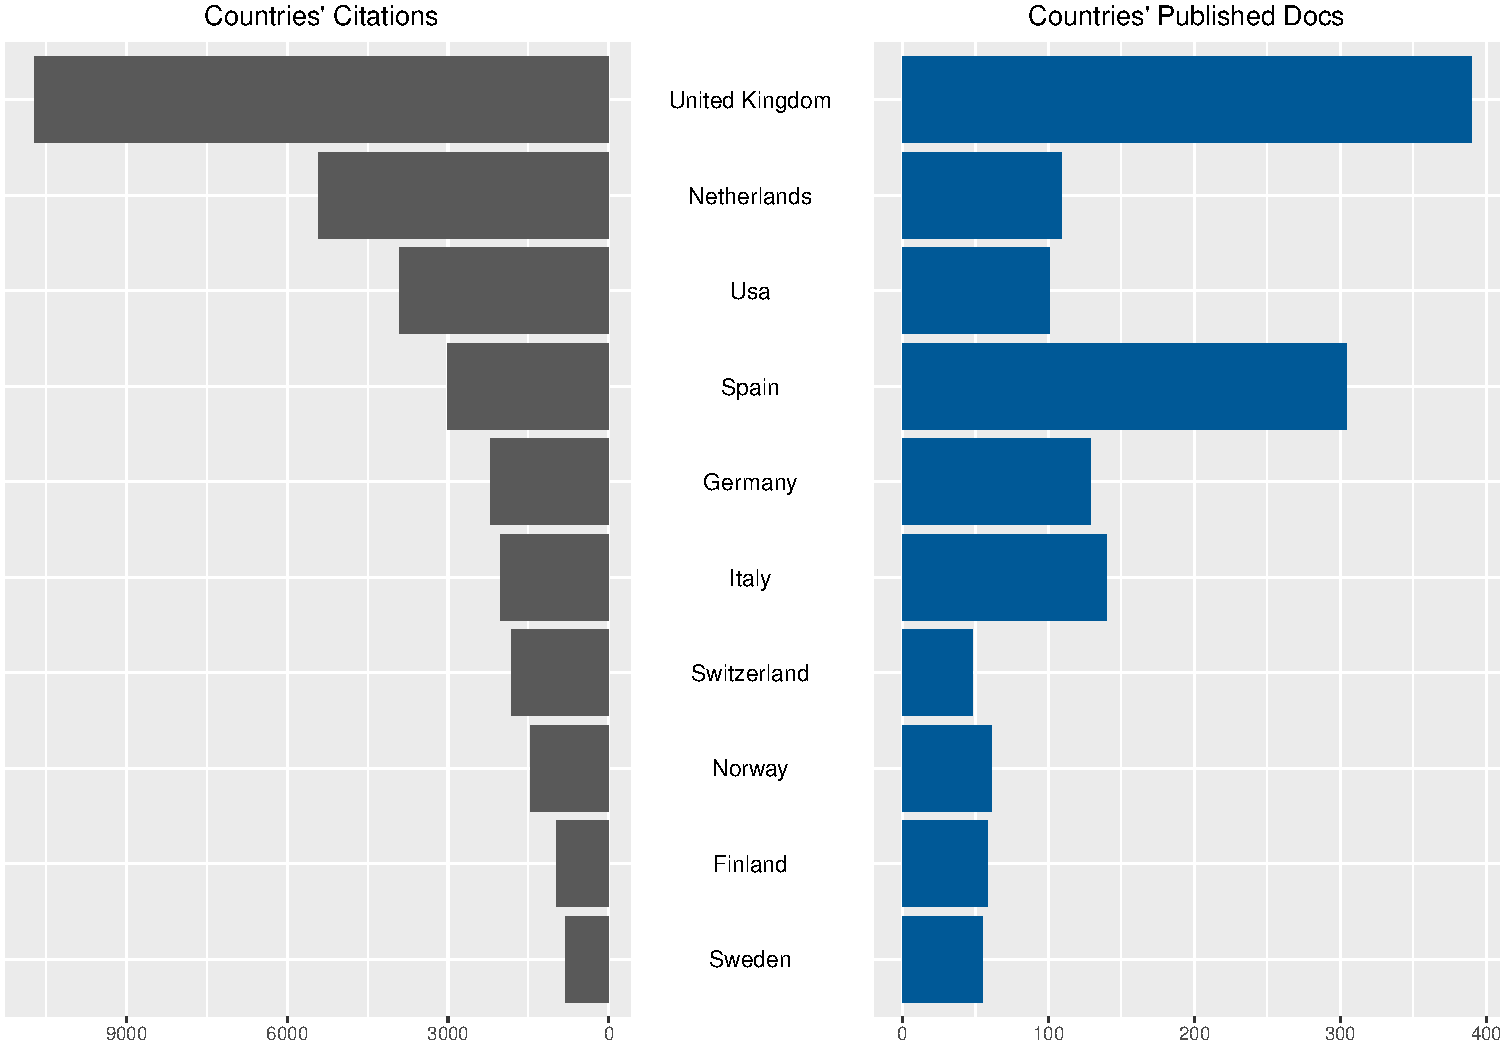
\includegraphics{Presentation_bibliometric_files/figure-beamer/Influencial CO-1.pdf}
\end{block}
\end{frame}

\begin{frame}{7. Science Mapping I}
\protect\hypertarget{science-mapping-i}{}
\begin{block}{7.1. Citation Analysis}
\protect\hypertarget{citation-analysis}{}
\begin{table}[!h]

\caption{\label{tab:Most cited refs}Most Cited References}
\centering
\fontsize{5}{7}\selectfont
\begin{tabular}[t]{r|p{9cm}|r}
\hline
\textbf{Rank} & \textbf{Article} & \textbf{TC}\\
\hline
1 & Norris P (2001) -Digital Divide Civic Engagement, Information Poverty, And The Internet Worldwide & 204\\
\hline
2 & Van Dijk J (2005) -The Deepening Divide: Inequality In The Information Society & 172\\
\hline
3 & Hargittai E (2002) -Second-Level Digital Divide: Differences In People's Online Skills & 136\\
\hline
4 & Van Dijk J (2006) -Digital Divide Research, Achievements And Shortcomings & 129\\
\hline
5 & Van Dijk J, Hacker K (2003) -The Digital Divide As A Complex And Dynamic Phenomenon & 114\\
\hline
6 & Selwyn N (2004) -Reconsidering Political And Popular Understandings Of The Digital Divide & 108\\
\hline
7 & Dimaggio P, Hargittai E, Celeste C, Shafer S (2004) -From Unequal Access To Differentiated Use: A Literature Review And Agenda For Research On Digital Inequality & 105\\
\hline
8 & Van Deursen A, Van Dijk J (2014) -The Digital Divide Shifts To Differences In Usage & 103\\
\hline
9 & Zillien N, Hargittai E (2009) -Digital Distinction: Status-Specific Types Of Internet Usage & 82\\
\hline
10 & Hargittai E, Hinnant A (2008) -Digital Inequality: Differences In Young Adults' Use Of The Internet & 80\\
\hline
\multicolumn{3}{l}{\textsuperscript{1} Source: Author's elaboration}\\
\multicolumn{3}{l}{\textsuperscript{2} TC: Times Cited}\\
\end{tabular}
\end{table}
\end{block}

\begin{block}{Similarity measures}
\protect\hypertarget{similarity-measures}{}
Following \citet{kammerer2021}

\begin{itemize}
\item
  \textbf{Research base:} cluster of academic publications in a research
  field that are considered fundamental to the development and
  understanding of the field.
\item
  \textbf{Research front:} cluster of academic publications that refers
  to emerging active areas of research considering themselves with a
  similar unsolved research problem.
\end{itemize}

\begin{center}
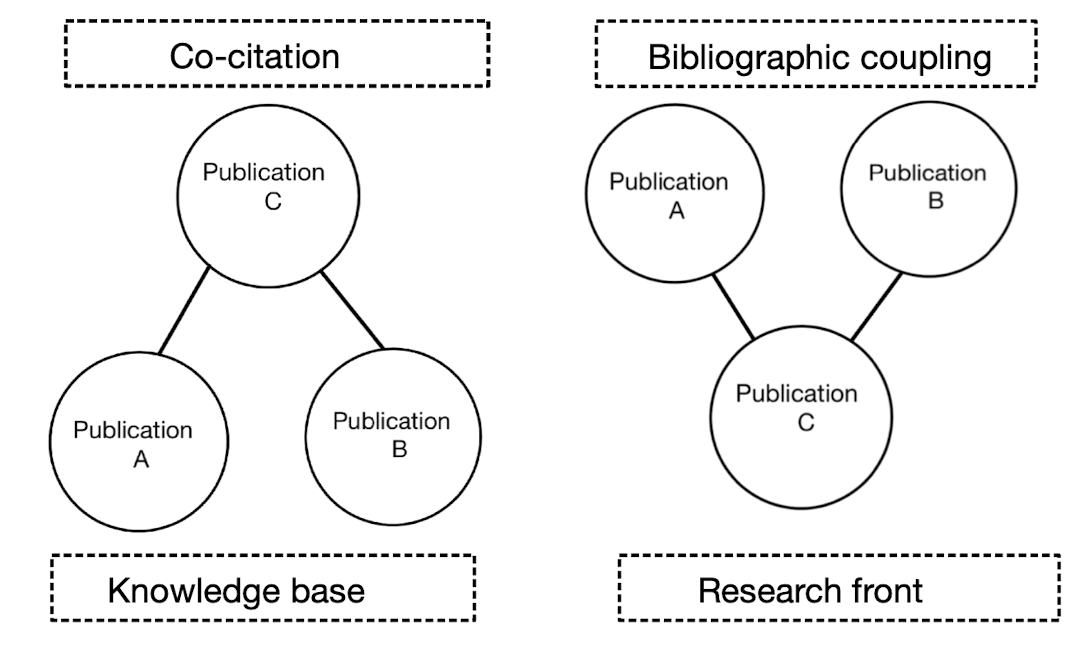
\includegraphics[width=0.6\textwidth]{pic_1.png}
\end{center}
\end{block}
\end{frame}

\begin{frame}{7. Science Mapping}
\protect\hypertarget{science-mapping}{}
\vspace{0.5cm}

\begin{block}{Co-citations Analyisis}
\protect\hypertarget{co-citations-analyisis}{}
This network shows the emergence of the literature on the digital divide

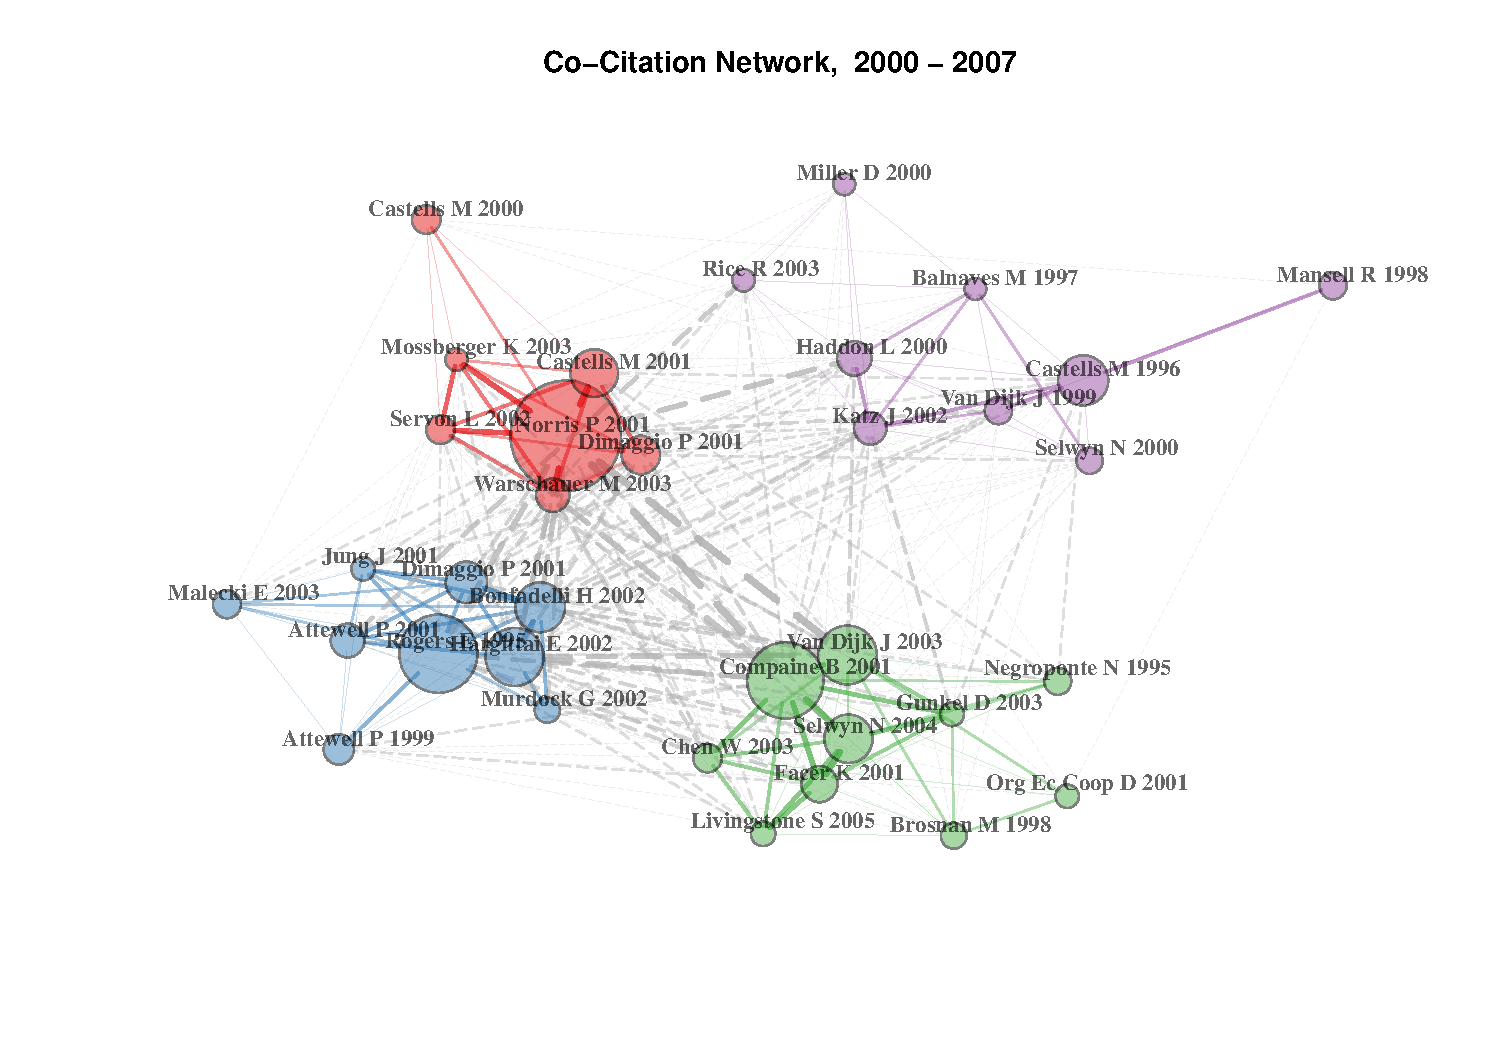
\includegraphics{Presentation_bibliometric_files/figure-beamer/Co_cite_P1-1.pdf}
\end{block}
\end{frame}

\begin{frame}{7. Science Mapping II}
\protect\hypertarget{science-mapping-ii}{}
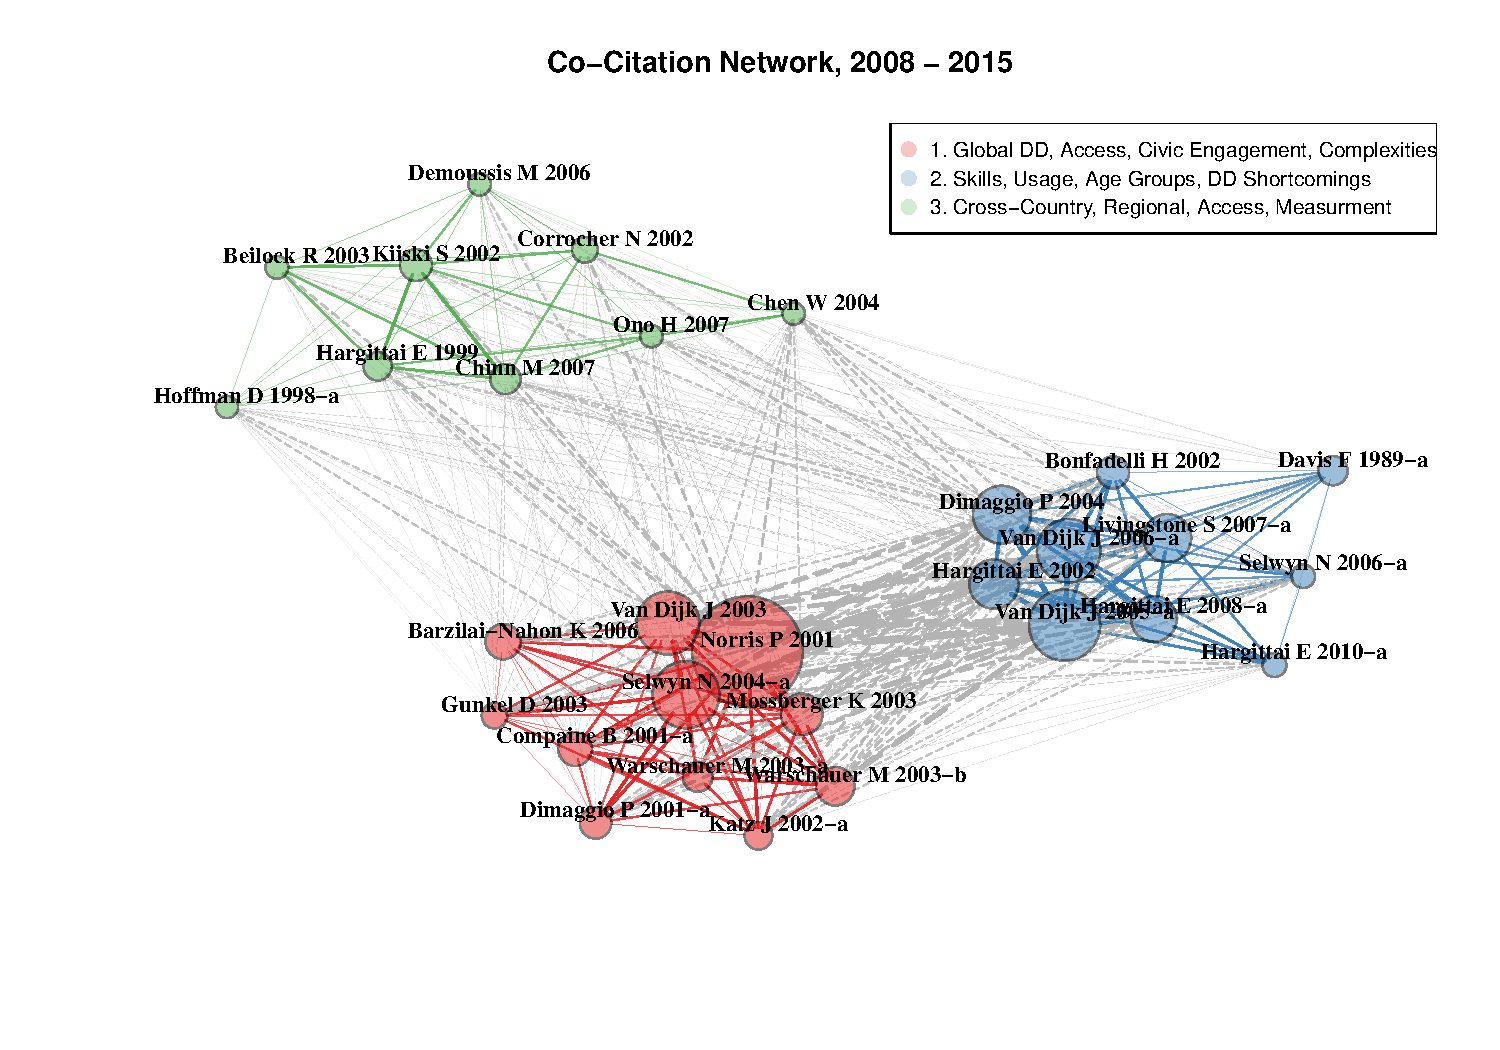
\includegraphics{Presentation_bibliometric_files/figure-beamer/Co_cite_P2-1.pdf}
\end{frame}

\begin{frame}{7. Science Mapping III}
\protect\hypertarget{science-mapping-iii}{}
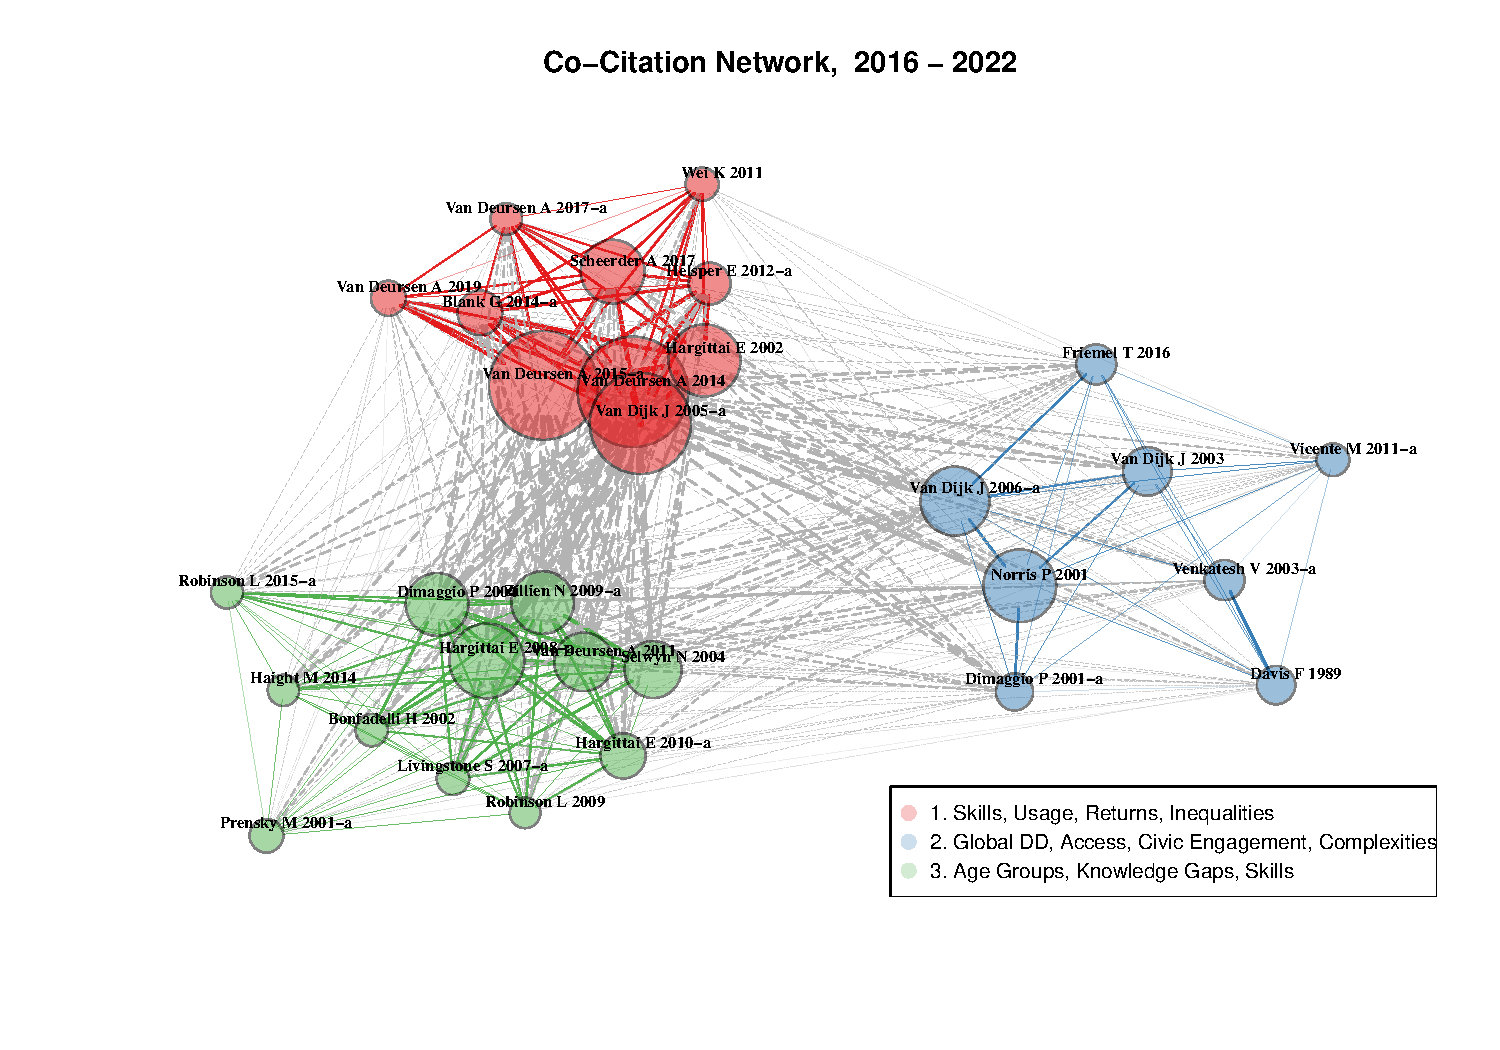
\includegraphics{Presentation_bibliometric_files/figure-beamer/Co_cite_P3-1.pdf}
\end{frame}

\begin{frame}{7. Science Mapping IV}
\protect\hypertarget{science-mapping-iv}{}
\end{frame}

\renewcommand\refname{References}
\begin{frame}[allowframebreaks]{References}
  \bibliographytrue
  \bibliography{references.bib}
\end{frame}

\end{document}
